%%%%%%%%%%%%%%%%%%%%%%%%%%%%%%%%%%%%%%%%
%%% master document for tcre.tex
%%%%%%%%%%%%%%%%%%%%%%%%%%%%%%%%%%%%%%%%

%%% class
\documentclass{article}

%%%%%%%%%%%%%%%%%%%%
%%% preamble
%%%%%%%%%%%%%%%%%%%%

%%% font encodings
\usepackage[T1]{fontenc}
\usepackage[utf8]{inputenc}
\usepackage{lmodern}

%%% bibliography
\usepackage[
  backend=biber,
  style=nature,
  natbib=true,
  url=false,
  doi=false,
  isbn=false,
  eprint=false,
  sorting=none
]{biblatex}

\addbibresource{Bibliography/auto.bib}
\addbibresource{Bibliography/byhand.bib}

%%% revision information
\usepackage[mark]{gitinfo2}
\renewcommand{\gitMark}{Branch: \gitBranch @\gitAbbrevHash \gitDirty\ \textbullet{} Author: \gitAuthorName\,(\gitAuthorIsoDate) \textbullet{} Tags: \gitTags}
\renewcommand{\gitMarkFormat}{\small}

%%% clicakable colored links
\usepackage{xcolor}
\usepackage[colorlinks=true,
  linkcolor=blue,
  urlcolor=blue,
  citecolor=blue,
  anchorcolor=blue
]{hyperref}

%%% nicier charater proturution, kerning, etc.
\usepackage{microtype}

%%% more math symbols
\usepackage{amsmath}
\usepackage{mathpazo}
%\usepackage{textgreek}

%%% proper fomating of units
\usepackage{siunitx}

%%% better tables
\usepackage{booktabs}

%%% generate tables from csv files
\usepackage{pgfplotstable}

%%% red colored margin notes
\usepackage{marginnote}
\renewcommand*{\marginfont}{\color{red}\sffamily}

%%% fancy author formating
\usepackage[affil-it]{authblk}

%%% title
\title{Two-Component Reference Energy for the Design of Proteins and Foldamers}

%%% authors & affiliations
\author[1]{Riley Simmons-Edler}
\author[2]{Andrew Watkins}
\author[2]{Paramjit Arora}
\author[1,2,3]{Richard Bonneau}
\author[1,3]{P. Douglas Renfrew\thanks{pdrenfrew@simonsfoundation.org}}
\affil[1]{Center for Genomics and Systems Biology, Department of Biology, New York University, New York, NY 10009, United States}
\affil[2]{Department of Chemistry, New York University, New York, NY 10003, United States}
\affil[3]{Simons Center for Data Analysis, Simons Foundation, New York, NY 10010, United States}

%\author{Riley Simmons-Edler \and P. Douglas Renfrew \and Andrew Watkins \and Paramjit Arora \and Richard Bonneau\thanks{Author order not finalized}}

%%% date
\date{}

%%%%%%%%%%%%%%%%%%%%
%%% document
%%%%%%%%%%%%%%%%%%%%
\begin{document}

\maketitle

%%% abstract
\begin{abstract}
  Algorithms for the design of biomacromolecules employ "reference energies" to correctly weight the probability of designing particular residue types. In the context of canonical amino acids, these quantities are typically treated as free parameters optimized to reproduce native sequences. More general methods exist to produce reference energies for non-canonical amino acids that provide a proxy for the energy of that residue type in an "unfolded" state. In this work, we develop an extension of these general methods that considers the "unfolded" state's single-residue score terms combined with inter-residue score terms derived from high-quality protein structures. In so doing, we produce a reference energy that yields sequence recovery comparable to the canonical-only framework but that possesses a clear physical basis, and which is entirely extensible to non-canonical amino acids and other foldamer residues.
\end{abstract}


%%% toc
\tableofcontents

%%% demo
\section{Demo}
This section demonstates how to do things in this document.
There are a few things that make working collaborativly on a large document easier.
First, \textit{\textbf{please keep a single sentence per line in the \TeX\ files.}}
This makes using version control easier since a small change doesn't look like an entire paragraph changed.
Second, \texttt{git diff -{}-word-diff} is a really nice tool for gettting differences between text documents rather than source code.

\subsection{Quotations}
Modern editors, like Micrsoft Word, try to infer the begining and ends of of quotes to so that the proper formating of the quotation marks can be used. For example, ``test'' and `test' are correct, "test" and 'test' are not.
They call this feature ``smart quotes.''
Latex requires you to be explicite using \texttt{`{}`word'{}'} (back-tic, back-tic, <word>, single-quote, single-quote) rather than \texttt{"word"} (double-quote, <word>, double-quote).
Smarter editors, like Emacs, do this automagically.

%\subsection{Equations}
%Here is an example equation that uses the equation enviroment and inline equations.
%stole this for the methods section to explain how Rosetta scoring works.

\subsection{Tables}
An example table is shown in Table~\ref{supptbl:rot_lib_snpshot_nmeo}.
This also shows how to reference tables and figures.

\begin{table}
  \centering
  \caption{Rotamers produced by the KMC or QMS rotamer library creation protocols for the NPHE peptoid side chain for a preceding-$\omega$, $\phi$, and $\psi$ of \ang{0}, \ang{-90}, \ang{180}}
  \label{supptbl:rot_lib_snpshot_nmeo}
  \begin{tabular}{rrrcrrr}
    \toprule
    \multicolumn{3}{c}{KMC} && \multicolumn{3}{c}{QMS} \\
    \cmidrule{1-3} \cmidrule{5-7}
    Prob & $\chi_1$  & $\chi_2$ && Prob & $\chi_1$  & $\chi_2$ \\
    \midrule
    0.98 & \ang{100}  &  \ang{88}  && 0.71 & \ang{82}  &  \ang{-116} \\
    0.01 & \ang{103}  &  \ang{-39} && 0.29 & \ang{-91} &  \ang{-71}  \\
    0.01 & \ang{-92}  &  \ang{107} && ~ & ~ & ~ \\
    0.00 & \ang{-142} &  \ang{52}  && ~ & ~ & ~ \\
    \bottomrule
  \end{tabular}
\end{table}

\subsection{Bibliography}
There will be two bibliography files: \texttt{auto.bib} and \texttt{byhand.bib}.
The former will contain an auto-generated bibliography file exported from a reference manager.
The later is for references that are difficult to get in to the reference manager (eg.~Gaussian).
If you have any papers you want to add, send them to me and I will add them to my reference manager and update the file.
Here are two example citations\cite{jacak_computational_2012,renfrew_incorporation_2012}.

\subsection{Notes}
I have added the \textsf{marginnote} package so that we can add littel notes in the margin.\marginnote{A little note/comment in the margin.}


%%% sections
\section{Introduction}
\subsection{Computational design of proteins and peptidomemetics}
The computational design of macromolecules like proteins has permitted dramatic advances in chemical and synthetic biology.
Protein design has resulted in advances in basic knowledge, such as the creation of proteins with novel folds\cite{kuhlman_design_2003}, as well as industrial and medical applications, such as the creation and optimization of enzymes that can conduct reactions that are not performed by natural enzymes\cite{jiang_denovo_2008,rothlisberger_kemp_2008}.

In recent years, the potential to extend existing peptide design methods to chemically diverse groups of heteropolymer molecules which display peptide-like properties such as secondary and tertiary structure.
Examples include peptoids\cite{renfrew_incorporation_2012}, oligo-oxopiperazines\cite{lao_rational_2014}, and $\beta$-peptides\cite{molski_remodeling_2012}, among others.
These molecules are an attractive alternative to peptides for drug design due to their high bioavailability, resistance to proteolysis, and ability to bind competitively at protein binding sites with high affinity by mimicking the conformation of the natural binding partner\cite{lao_rational_2014}.
Similarly, incorporating non-natural side chains in peptides may yield increases in binding affinity and specificity as well as protein stability relative to proteins containing only the canonical twenty amino acids\cite{horng_values_2003}.

Proteins and peptides containing only the canonical amino acids can be optimized for a variety of applications with Rosetta\cite{leaver-fay_chapter_2011,jiang_denovo_2008,rothlisberger_kemp_2008,raveh_scheuler_furman_2011}.
The incorporation of non-canonical amino acids (NCAAs) and peptidomimetics is ongoing.
While it is now possible to design with a variety of NCAAs in Rosetta\cite{renfrew_incorporation_2012,drew_adding_2013}, NCAA design still faces several issues in practice which make it difficult to apply to many problems.
Chief among these is the difficulty in correcting for the statistical and energetic biases towards certain residue types that result from Rosetta's sampling methods and energy model.

\subsection{Rosetta design and the need to adjust for statistical bias}
Unlike continuous transformations to a protein structure, such as altering internal coordinates, changes in sequence are discrete.
Within Rosetta, each side chain is represented as a rotational isomer called a rotamer.
Therefore, changes in sequence are accomplished via rotamer substitution; a protein or peptide may be redesigned by repacking its sidechains while permitting those residues to change their amino acid identity\cite{leaver-fay_chapter_2011}.

One issue with this state-based approach is that design moves that would substitute a residue with many $\chi$(chi) angles are relatively disfavored. For example, in any particular protein conformation, relatively few of lysine's 81 rotamers are energetically favorable.
As a result, these residues tend to be excessively unfavorable in design\cite{leaver-fay_chapter_2013,rohl_protein_2004}.
An additional scoring term, called a reference energy, can be incorporated for every amino acid to account for this bias.
In the Rosetta canonical amino acid scoring function, this reference energy term is called \textit{ref} and consists of a series of 20 weights, one for each canonical amino acid.
These weights are trained to maximize sequence recovery on a set of protein crystal structures.
Without this term, Rosetta suffers from reduced sequence recovery in native proteins, as well as highly imbalanced design frequencies\cite{rohl_protein_2004}.

\subsection{The existing noncanonical reference energy in Rosetta}

While this statistical weighting works well for canonical amino acid types for which an ideal native residue frequency exists, NCAAs and peptidomemetics cannot benefit from a statistically derived reference energy or sequence recovery benchmark.
The initial incorporation of NCAAs into Rosetta featured the development of the \textit{unfolded} energy term, which took the place of the canonical reference energy\cite{renfrew_incorporation_2012}.
The \textit{unfolded} energy was created by taking native 5-mer fragments and mutating the central residue to the desired residue type; the average energy would thus reflect an intrinsic energetic expectation for that residue type.
Using the \textit{unfolded} term, the non-canonical scoring function \textit{mm\_std} was able to achieve useful levels of sequence recovery.

The unfolded state energy has enabled the design and synthesis of NCAA-containing peptides and peptidomimetics\cite{lao_rational_2014,drew_adding_2013}, but it can be improved in several ways.
First, it relies on fragments from natural peptides, which have backbone angles that may not correlate well to non-peptidic scaffolds like the oligo-oxopiperazine.
Second, it is not impossible to mutate the central residue of a 5-mer fragment to a $\beta$-amino acid due to its additional backbone atom.
Third, the average score of a typical 5-mer fragment possesses a very small attractive term and a relatively large solvation penalty, because few fragment residues contact the central side-chain.
Thus, the \textit{unfolded} energy tends to favor large, hydrophobic residues: even solvent-exposed positions, which ordinarily are quite polar in nature, may be redesigned to tryptophan because their \textit{unfolded} score already possesses a large desolvation penalty.

The two-component reference energy (TCRE) addresses each of these issues.
The TCRE improves upon the existing $unfolded$ term for NCAAs; it additionally could replace or supplement the statistical \textit{ref} term for use with the canonical scoring function.

\section{Methods}

\subsection{Rosetta scoring functionality and relevant score functions}
\paragraph{}
Rosetta uses multiple scoring functions for evaluating macromolecule structures, called poses, in different contexts.
Each score function is a weighted sum of scoring terms that describe some energetic property of the pose.
These energy terms are either physically or statistically derived and may be functions of one or two atoms or residues.
The individual weights, $W_x$, on each energy term are typically fit using a special protocol called OptE\cite{leaver-fay_chapter_2013}.

The Rosetta scoring function can be expressed as in equation \ref{equ:rosetta_sum_of_terms}, where \textit{n} is the total number of residues, $W_{x}$ is the weight on energy term \textit{x} (eg.\ \textit{fa\_rep}, \textit{fa\_sol}, etc.), $E_{x,i}$ is the energy for energy term \textit{x} for the residue at position \textit{i}.

\begin{equation}
  \label{equ:rosetta_sum_of_terms}
  E_{\text{pose}} = \sum_{i}^{n_{\text{res}}} W_{x} E_{x,i} + ... + W_{y} E_{y,i}
\end{equation}

\paragraph{}
% I hate the phrase "designed for general purpose protein evaluation" but I'm not sure of a better successor. Really, I just want to say that it's only compatible with canonical amino acids...
Rosetta protocols most frequently use the scoring function \textit{talaris2013}, which was designed for general purpose protein evaluation using canonical amino acids\cite{leaver-fay_chapter_2013}.
It consists of the score terms \textit{fa\_atr}, \textit{fa\_rep}, \textit{fa\_sol}, \textit{fa\_elec}, \textit{fa\_intra\_rep}, \textit{pro\_close}, \textit{hbond\_sr\_bb}, \textit{hbond\_lr\_bb}, \textit{hbond\_bb\_sc}, \textit{hbond\_sc}, \textit{dslf\_fa13}, \textit{rama}, \textit{omega}, \textit{fa\_dun}, \textit{p\_aa\_pp}, and \textit{ref}.
Full descriptions of these energy terms can be found in \cite{leaver-fay_chapter_2013}.
%optionally include descriptions of these terms here.

\paragraph{}
The scoring function \textit{mm\_std} is available to model structures that include NCAAs and peptidomimetics, called \cite{renfrew_incorporation_2012}.
The energy terms of this score function are \textit{fa\_atr}, \textit{fa\_rep}, \textit{fa\_sol}, \textit{mm\_lj\_intra\_atr}, \textit{mm\_lj\_intra\_rep}, \textit{mm\_twist}, \textit{pro\_close}, \textit{hbond\_sr\_bb}, \textit{hbond\_lr\_bb}, \textit{hbond\_bb\_sc}, \textit{hbond\_sc}, \textit{dslf\_ss\_dst}, \textit{dslf\_cs\_ang}, \textit{dslf\_ss\_dih}, \textit{dslf\_ca\_dih}, and \textit{unfolded}.
\textit{mm\_std} lacks the statistical potentials used by \textit{talaris2013}, such as \textit{p\_aa\_pp}, which derives from the probability that a given residue type is found at a given point in Ramachandran space.
Since such statistical potentials are not available for NCAAs in general, the molecular mechanics potentials are included to compensate.
Crucially, \textit{mm\_std} replaces \textit{ref} with an explicit energetic model of the unfolded state of each residue, called \textit{unfolded}.

\subsection{The structure of the two-component reference energy}
\paragraph{}
The two-component reference energy (TCRE) addresses the aforementioned shortcomings of $unfolded$ by treating the one- and two-body energies of a residue separately.
By evaluating the two-body scoring terms in the context of folded proteins, the TCRE eliminates any bias towards large residues.
By evaluating one body energies in the context of an acetylated, methylamidated dipeptide, the TCRE avoids any context-dependent issues of scoring
Each residue type possesses a one body energy and a two body energy derived from the summed two body scores of its constituent atom types.
The relative weights of those components are free to be optimized.
% I find the below statement far too vague and speculative. -amw
%In addition, the method can be applied to arbitrary peptides and peptidomimetics by dynamically constructing residue reference energies from constituent atomic energies in response to the residue types in use, which allows the method to be extended to theoretically arbitrary molecules in Rosetta.

\subsection{Generating per-atom-type two-body energy distributions}
\paragraph{}
The "two-body" component of the split unfolded energy is derived from examining the distribution of individual two-body scoring terms over all the occurrences of a given atom type in a high quality set of protein structures.
To evaluate the effect of our choice of "atom type" set, we examined both the modified CHARMM atom type set used by Rosetta\cite{leaver-fay_chapter_2011,bernard_charmm_1983} and the molecular mechanics (MM)-based atom types\cite{renfrew_incorporation_2012}. % Doug--these are also CHARMM derived, right? How should we phrase the distinction?
As limiting cases, we considered elemental types, where all atoms of the same element are alike, as well as unique atom types, where every atom of every residue type is treated differently.
The Top8000 benchmark set of high quality structures\cite{lovell_structure_2003} provides around $10^6$ examples of most atom types. These structures were scored with Rosetta using a modified protocol that recorded every inter-atomic energy value for the scoring terms \textit{fa\_atr}, \textit{fa\_rep}, \textit{fa\_sol}, \textit{fa\_elec}, \textit{hbond}, and \textit{dslf\_fa13}.
These inter-atomic energies were evaluated on each example of each atom type, and a measure of centrality was extracted from the resulting distribution.

%Table to illustrate the differences between the atom type sets.
\begin{table}
  \centering
  \caption{The four atom type sets categorize the above examples of carbon atoms commonly found in protein structures quite differently.}
  \label{tab:atypes_example}
  \begin{tabular}{clllll}
    \toprule
    Residue & Atom Name & Elemental Type & Rosetta Type & MM Type & Unique Type\\
    \midrule
    GLY & $\alpha$-Carbon & C & CAbb & CT1 & GLY/2\\
    ALA & $\alpha$-Carbon & C & CAbb & CT1 & ALA/2\\
    ALA & $\beta$-Carbon & C & CH3 & CT3 & ALA/5\\
    ALA & Carboxyl Carbon & C & CObb & C & ALA/3\\
    %Perhaps two more that differentiate Rosetta and MM?
    \bottomrule
  \end{tabular}
\end{table}

\paragraph{}
We evaluated the mean, median, mode, and Boltzmann-weighted average as central measures for each scoring term.
The median exhibited a slight advantage in sequence recovery benchmarks (FIGURE?!) and was used in all further testing.

\subsection{Atom types only found in NCAAs}
\paragraph{}
A limited number of atom types found in NCAAs currently implemented in Rosetta are not found in canonical amino acids, and thus cannot be scored using the Top8000 data set.
To obtain expected energy distributions for these atom types, which include e.g. the halogens, we mutated all instances of a canonical residue type to a noncanonical analogue that includes the atom type in question and performed limited rotamer repacking and mimimization to resolve clashes.
We analyzed the resulting scoring term distributions in the same way.
Table \ref{tab:atypes_all} describes the molecular mechanics atom types which had to be evaluated in this way.


%Probably want to trim this to just NCAA atom types and/or move it to the supplement...
\begin{table}
  \caption{MM atom types found only in NCAAs for which two body energies were obtained.}
  \label{tab:atypes_all}

%\begin{tabular}{c|lll}
%Atom Type Set & Atom Type & Natural?\\
%\hline
%Elemental & C & yes\\
%Elemental & O & yes\\
%Elemental & H & yes\\
%Elemental & N & yes\\
%Elemental & S & yes\\
%\hline
%Rosetta & HNbb & yes\\
%Rosetta & Ntrp & yes\\
%Rosetta & aroC & yes\\
%Rosetta & ONH2 & yes\\
%Rosetta & Narg & yes\\
%Rosetta & COO & yes\\
%Rosetta & CH1 & yes\\
%Rosetta & CH2 & yes\\
%Rosetta & CH3 & yes\\
%Rosetta & OCbb & yes\\
%Rosetta & NH2O & yes\\
%Rosetta & Nlys & yes\\
%Rosetta & CAbb & yes\\
%Rosetta & S & yes\\
%Rosetta & Nhis & yes\\
%Rosetta & Npro & yes\\
%Rosetta & Haro & yes\\
%Rosetta & CNH2 & yes\\
%Rosetta & OOC & yes\\
%Rosetta & OH & yes\\
%Rosetta & Hpol & yes\\
%Rosetta & CObb & yes\\
%Rosetta & Nbb & yes\\
%Rosetta & Hapo & yes\\
%\hline
%Rosetta & Cl & no\\
%Rosetta & I & no\\
%Rosetta & Br & no\\
%Rosetta & F & no\\
%\hline
  \begin{tabular}{c|l}
    \toprule
    Atom Type & description\\
    \midrule
%HS & yes\\
%NC2 & yes\\
%NR2 & yes\\
%HB & yes\\
%HC & yes\\
%NR1 & yes\\
%HA & yes\\
%CPT & yes\\
%HR1 & yes\\
%HR3 & yes\\
%NY & yes\\
%HP & yes\\
%C & yes\\
%CC & yes\\
%CA & yes\\
%H & yes\\
%CA & yes\\
%O & yes\\
%N & yes\\
%S & yes\\
%NH1 & yes\\
%NH3 & yes\\
%NH2 & yes\\
%OH1 & yes\\
%CT1 & yes\\
%CT2 & yes\\
%CT3 & yes\\
%OC & yes\\
%CY & yes\\
%SM & yes\\
%CP1 & yes\\
%CP2 & yes\\
%CP3 & yes\\
%CPH1 & yes\\
%CPH2 & yes\\
%\hline
    BR & bromine\\
    CAP & aromatic carbon in pyridine ring\\
    CE1 & monosubstituted alkene carbon\\
    CE2 & terminal alkene carbon\\
    CF1 & monofluorinated carbon\\
    CF3 & trifluorinated carbon\\
    CL & chlorine\\
    F1 & fluorine on CH$_2$R\\
    F3 & fluorine on CF$_2$R\\
    HE1 & proton on monosubstituted alkene carbon \\
    HE2 & proton on terminal alkene carbon\\
    I & iodine\\
    OE & ether oxygen\\
    \bottomrule
  \end{tabular}
\end{table}


\begin{figure}
  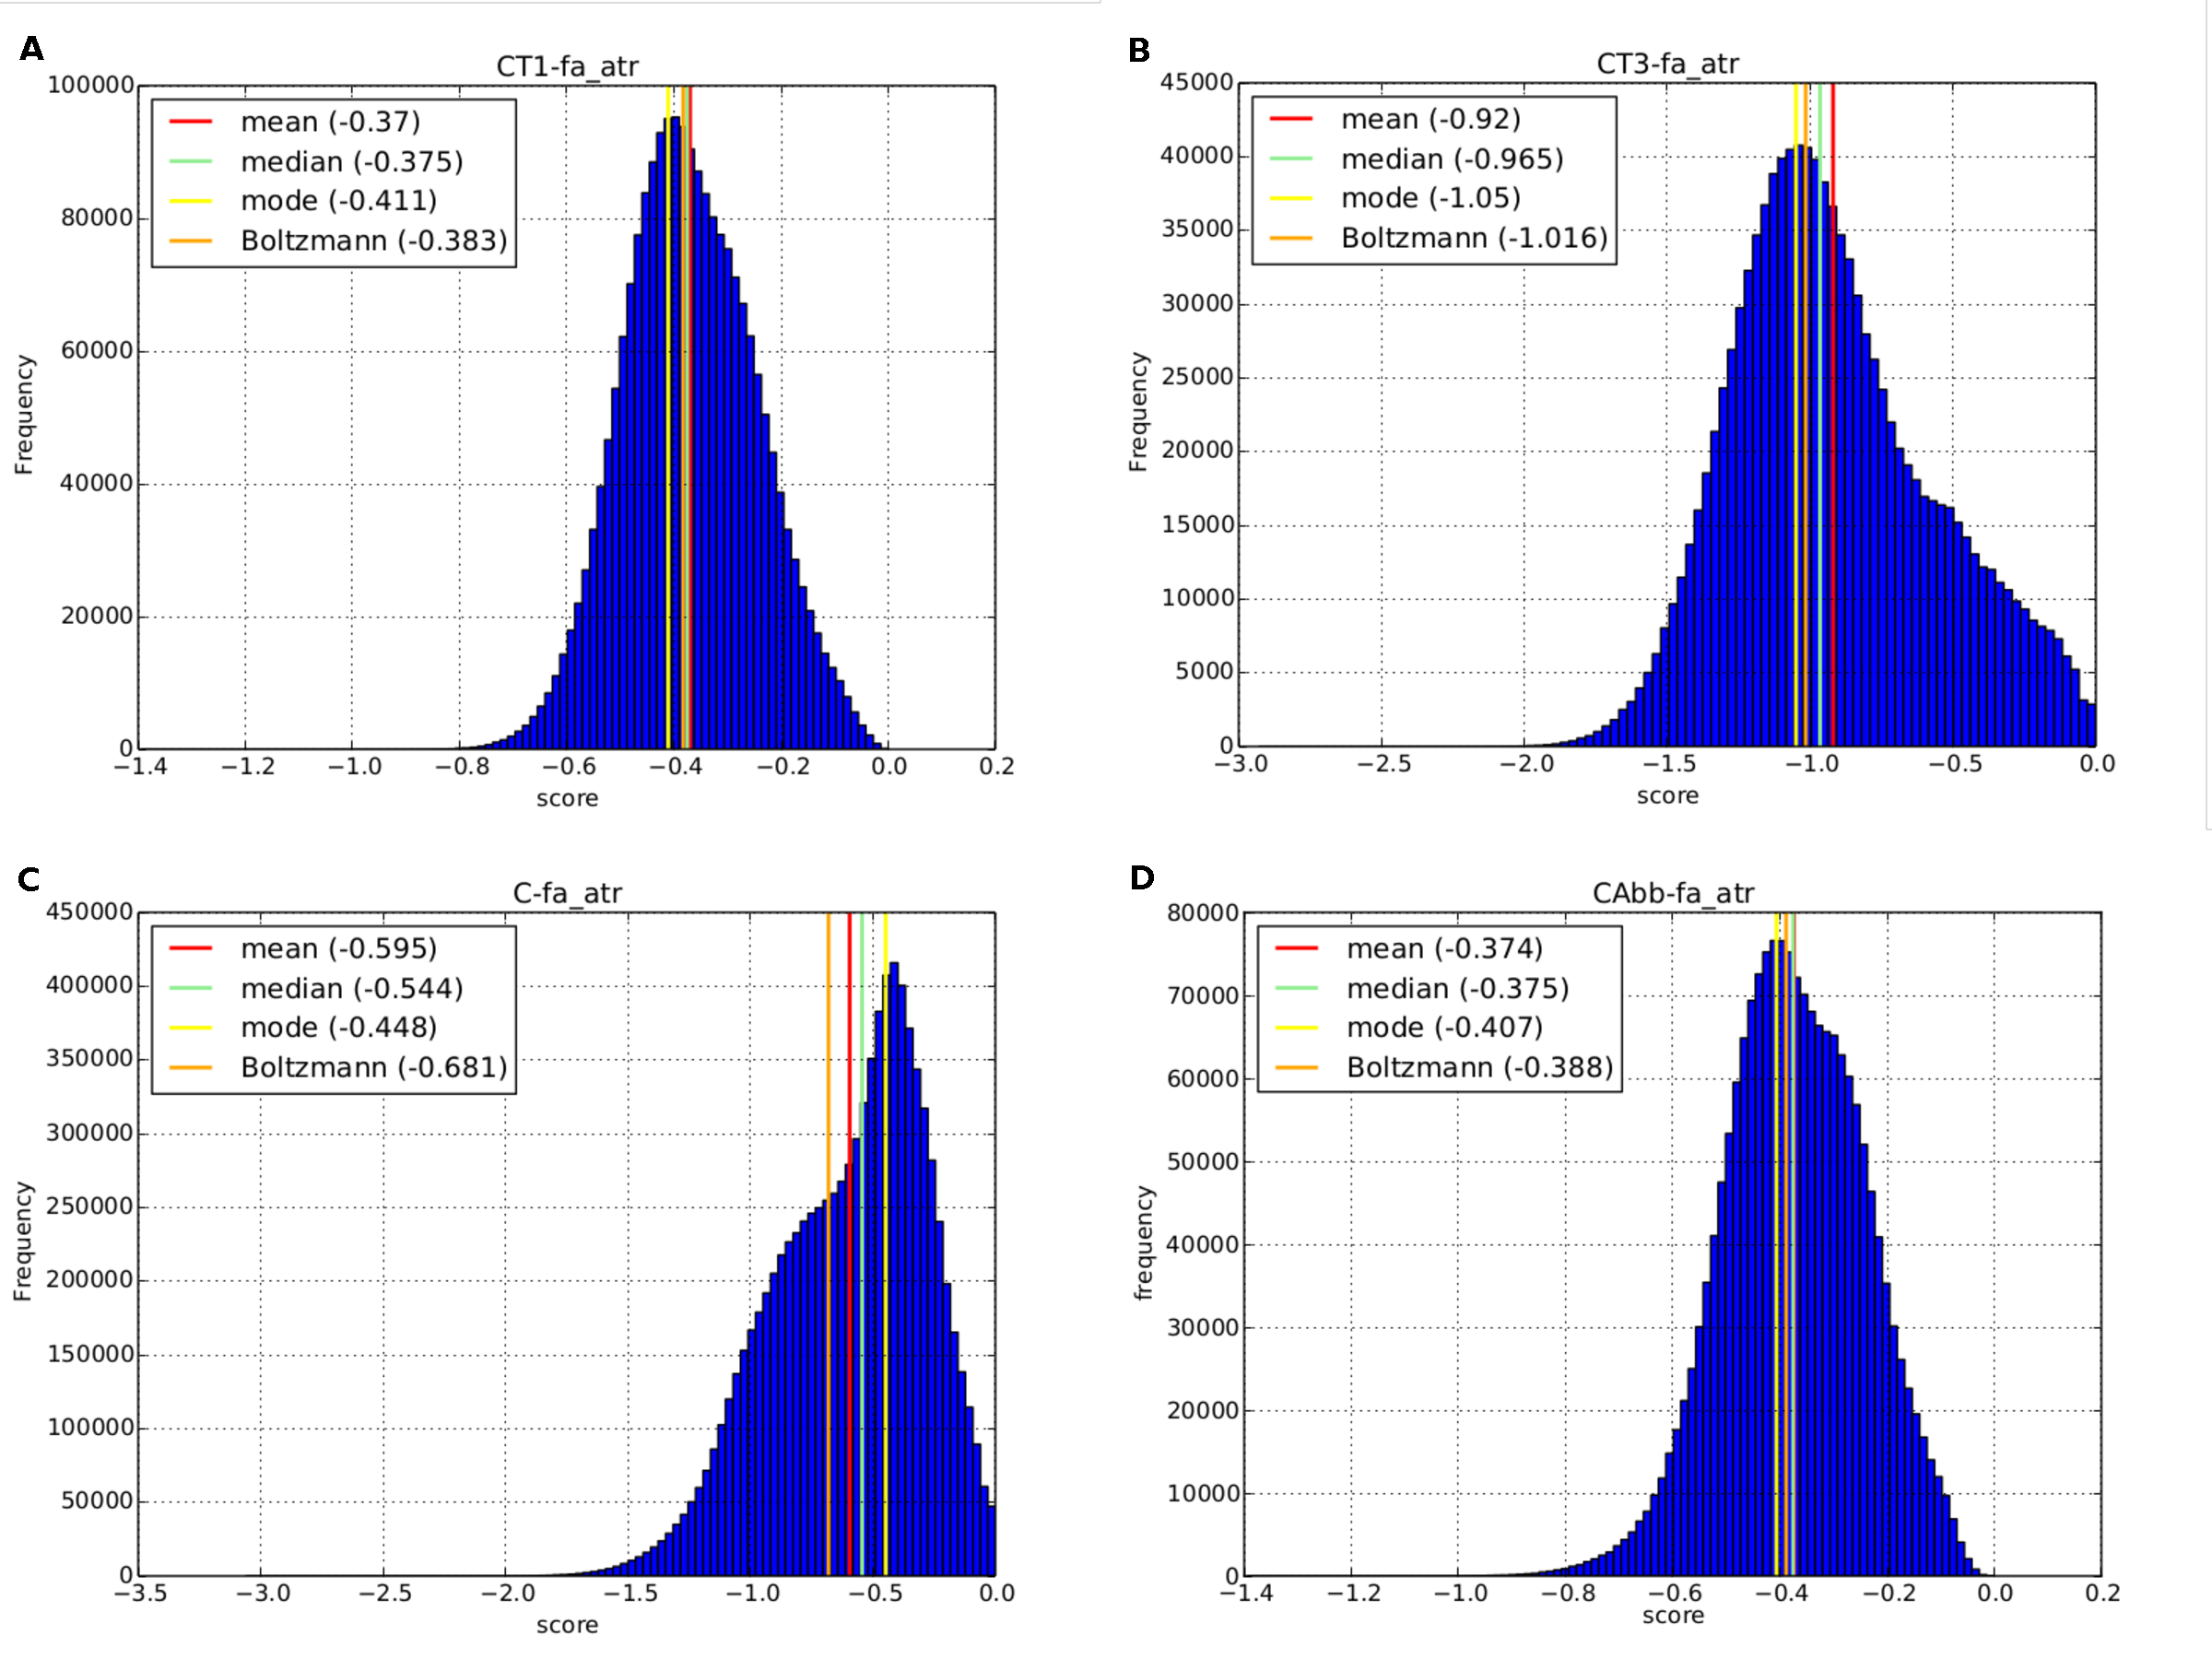
\includegraphics[width=\linewidth]{Figures/atom_energy_distribution_examples.pdf}
  \caption{Example histograms of the \textit{fa\_atr} Lennard-Jones attractive component energy term for several atoms in different atom sets.
    \textbf{A.} The molecular mechanics atom type CT1, a carbon with one hydrogen, and the atom type of the backbone $\alpha$-carbon, among other carbon atoms.
    \textbf{B.} The molecular mechanics atom type CT3, a methyl group, used in several amino acid sidechains.
    \textbf{C.} The elemental atom type C, carbon.
    \textbf{D.} The Rosetta atom type CAbb, the backbone $\alpha$-carbon.
    The median value shown by the green line is the representative value used to construct the amino acid two body energies.}
  \label{fig:tbaedist}
\end{figure}


%\subsection{Formulation of the two component reference energy}
%\paragraph{}
%Our split unfolded energy function is composed of two scoring terms in Rosetta, a one body and a two body component.
%During scoring, each of these terms is calculated separately for each residue in the protein, and then weighted and summed similar to each other Rosetta energy term.
%This combined energy term serves to replace the standard Rosetta reference energy function, known as $ref$.
%The formulation of the two component reference energy for a protein, $E_{TCR}$, is thus:

%replaced with a better equation in a figure from Doug's Rosettacon 2014 poster.
%\begin{equation}
%  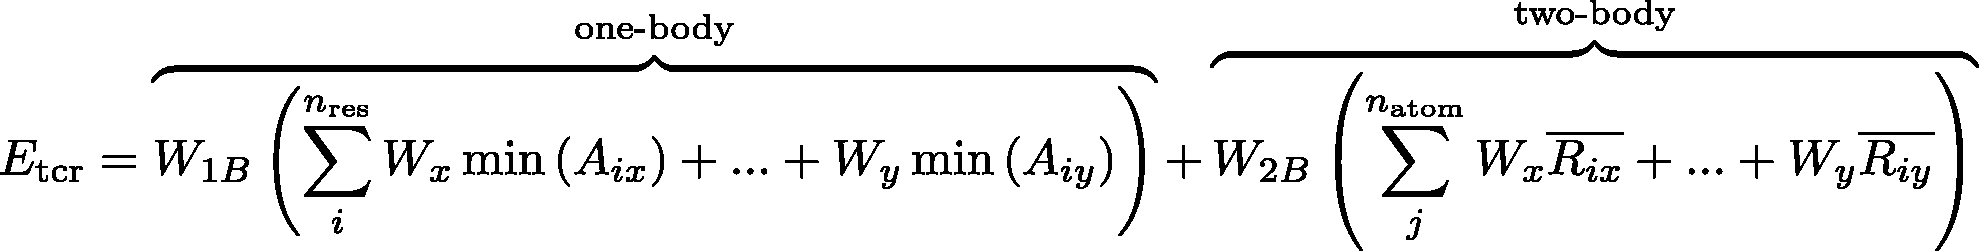
\includegraphics[width=0.9\linewidth]{Figures/tcr_equation.pdf}
%E_{\text{unfolded}} =  W_{1body} \sum_{i}^{n_{\text{res}}} E_{i,1body} +  W_{2body} \sum_{i}^{n_{\text{res}}} E_{i,2body}
%\end{equation}

%Where $W_{1B}$ is the weight placed on the one body term, $W_{2B}$ is the weight placed on the two body term, $min(A_{ix})$ is the minimal value for the one body energy term \textit{x} of the reference energy for residue \textit{i}, and $R_{jx}$ is the median two body energy term \textit{x} for residue \textit{j}.

%\subsection{Calculation of the two body energy term}
%\paragraph{}
%The two body portion of our two component reference energy consists of a sum of the energies of each constitutent atom.
%These atomic energies are calculated from instances of each atom type in the set used appearing in the top8000 data set of high-quality protein crystal structures, as described above.
%These values for each Rosetta score term calculated on a per-atom basis are stored in a lookup table, and per-residue two body unfolded energies are built dynamically as needed during runtime from these atom energy lookups.
%The two body reference energy for the protein is calculated as follows:

%\begin{equation}
%E_{\text{2body}} = W_{2body} \sum_{i}^{n_{\text{res}}} \sum_{j}^{l_{\text{scoreterms}}} W_{j} \sum_{k}^{m_{\text{atoms}}} E_{k}
%\end{equation}

%Where $W_{two-body}$ is the weight value for the two body term, \textit{n} is the total number of residues, \textit{l} is the score terms \textit{fa\_atr}, \textit{fa\_rep}, \textit{fa\_sol}, \textit{fa\_elec}, \textit{hbond}, and \textit{fa\_dslf13} for the \textit{talaris2013} scoring function and the score terms \textit{fa\_atr}, \textit{fa\_rep}, \textit{fa\_elec}, \textit{hbond}, and \textit{fa\_dslf13} for the \textit{mm\_std} scoring function, $W_{j}$ is the weight on score term \textit{j}, \textit{m} is the number of atoms in the residue \textit{i}, and $E_{k}$ is the energy of atom \textit{k} in the two body atom energy lookup table.


\subsection{Determining the single-body reference energy}
\paragraph{}
The one body component of the reference energy represents the minimum achievable energy of a given residue type for a given scoring function.
We prepended and appended acetyl and N-methylamide capping groups to the residue in question and iterated its backbone dihedral angles in one degree bins, followed by backbone minimization, sidechain repacking, and sidechain minimization.
The lowest energy conformation among those sampled was taken as the ideal conformation for that residue type.
The weighted sum of its intra-residue energies serve as the single-body component of the TCRE.
This process was carried out using the intra-residue scoring terms for both the \textit{talaris2013} score function and the \textit{mm\_std} score function.
For \textit{talaris2013}, the intra-residue terms are \textit{fa\_intra\_rep}, \textit{pro\_close}, \textit{fa\_dun}, \textit{rama}, \textit{omega}, and \textit{p\_aa\_pp}.
For \textit{mm\_std}, the intra-residue terms are \textit{mm\_lj\_intra\_rep}, \textit{mm\_lj\_intra\_atr}, \textit{mm\_twist}, and \textit{pro\_close}.

%\paragraph{}
%During runtime, the one body reference energy of a protein is determined by summing the values thus recorded for each residue type in it's sequence, which is then weighted and summed with the other score terms to produce the total energy of the protein.
%The formulation of the one body term for a given protein is described below.

%\begin{equation}
%E_{\text{1body}} = W_{1body} \sum_{i}^{n_{\text{res}}} \sum_{k}^{j_{\text{scoreterms}}} W_{k} %E_{restype_{i},k}
%\end{equation}

%Where $W_{1body}$ is the one body energy term weight, \textit{n} is the total number of residues, \textit{j} is the set of score terms used to compute the one body energy term for the current score function(either \textit{talaris2013} or \textit{mm\_std}), $W_{k}$ is the weight applied to score term \textit{k} under the energy function in use, and $E_{restype_{i},k}$ is the one body minimal energy value for the score term \textit{k} for the residue type of residue \textit{i} in the protein.


\subsection{Design Benchmarking via Sequence Recovery}
\paragraph{}
To test the utility of our two component reference energy for protein design, we used the Rosetta native sequence recovery benchmark protocol\cite{leaver-fay_chapter_2013}.
In this protocol, a collection of 41 high-quality protein structures are fully redesigned by Rosetta using a given scoring function.
Two qualities of the scoring function are tested: its ability to recapitulate the native amino acid at each position and its ability to recapitulate overall native amino acid frequencies.
Both metrics describe its ability to design ``natural-like'' protein sequences for a given structure.
To guide analysis, we categorized the twenty canonical amino acids as hydrophobic, polar, positively charged, and negatively charged, since residues in each category response similarly to individual scoring terms.
%These categories were hydrophobic amino acids, consisting of residues valine, isoleucine, leucine, methionine, phenylalanine, glycine, alanine, proline, tryptophan, and tyrosine, polar amino acids, consisting of residues serine, threonine, asparagine, and glutamine, positively charged amino acids, consisting of residues arginine, lysine, and histidine, and negatively charged amino acids, consisting of aspartic acid and glutamic acid.
Using \textit{ref}, the canonical reference energy, \textit{talaris2013} performs much better on hydrophobic amino acids, moderately well on polar amino acids, and much worse on positive and negative amino acids.
%While no benchmark set exists for the design of non-canonical residue types, performance on the canonical residue types should be indicative of performance on NCAA types as well, as these types are treated identically during runtime.

\section{Results}
SEQUENCE RECOVERY FIGURE

PLOT: OLD REFERENCE ENERGIES, ONE BODY TERM, NEW REFERENCE ENERGIES

PLOT: TWO BODY TERMS

PLOT: ONE SCORETERM HISTOGRAM

\subsection{One and Two Body Unfolded Energy Terms}
\paragraph{}
We developed and implemented in Rosetta two energy terms, $unfolded$ and $split\_unfolded\_two\_body$, which represent the one body and two body portions of the expected energy of a given residue type.
These terms are extensible and can be applied to novel residue types, including peptidomemetics containing exotic backbone elements, with a minimum of additional development, and we present them here with all 20 canonical amino acids and <some number> of NCAA residue types, listed in table <number>.
The implementation of additional NCAA types that use only atom types listed in table \ref{tab:atypes_all} for use with these energy terms is intended to be a simple process, requiring only the generation of a one body low energy score set.
While the details of doing this differ slightly when additional backbone degrees of freedom are added, for residue types with rotation around only psi and psi, an application is provided to generate these one body energies, found under $src/apps/public/rileyse/FindMinEnergyOfDipeptideAA.cc$ in the Rosetta code repository.
Usage details can be found in the methods section.

\paragraph{}
The $unfolded$ term we have implemented, while sharing much of it's code with the $unfolded$ score term implemented in 2012 Renfrew at al[ref], is distinct in function and generation from the older term.
The newer term consists of a sum of the intra-residue energy terms used in Rosetta for the residue in it's minimum energy dipeptide form(i.e. possessing capping acetyl and N-methyl groups to mimic adjacent backbone atoms), as a measure of the minimum energetic contribution of the residue to a folded protein structure.
The older term is an average energy of the residue when inserted as the central residue in a large number of five residue fragments from structured proteins, and includes two body energy terms as well, and is thus not directly comparable to this new $unfolded$ term.

\paragraph{}
The two body term $split\_unfolded\_two\_body$, meanwhile, is an average intra-residue energy for a given residue type taken from many instances in folded protein structures from the top8000 high quality protein structure benchmark[ref].
This term represents the expected two body energy of a residue in a folded protein context, and serves as a benchmark during design to tell how a designed instance of a residue type compares to the expected case, which is assumed to be a well satisfied instance of that residue type. 


\subsection{Modifications to the mm\_std score function}
\paragraph{}
In addition to our development of the split unfolded energy terms, we also made several revisions and updates to the $mm\_std$ score function, previously described by Renfrew et al in [ref], and which is currently the standard scoring function for non-canonical design tasks in Rosetta.
Since this score function was introduced, several significant updates to canonical protein scoring function were published with the introduction of the $talaris2013$ score function, which replaced $score12\_full$ as the standard Rosetta scoring function[ref-talaris2013].
Some of these updates could be easily ported over to $mm\_std$, specifically a proper electrostatics term, $fa\_elec$, which was previously lacking in $mm\_std$, and an updated disulfide bond term, $dslf\_fa13$.
To adapt these terms, we adjusted the weights used in the $talaris2013$ score function relative to the difference in specific weights between the two score function.
In the case of $fa\_elec$, we weighted it relative to the average of the hydrogen bonding score terms in $mm\_std$ versus those in $talaris2013$, which were slightly higher in $mm\_std$, resulting in a weight of 0.73 versus 0.70 for the $fa\_elec$ term in $talaris2013$.
In the case of the $dslf\_fa13$ term, the old disulfide bond score terms in $mm\_std$ were identical to those from $score12\_full$, and so the $talaris2013$ weight of 1.0 was used as-is.
The resulting score function weights file can be found in the Rosetta code repository as $/database/scoring/weights/mm\_std\_fa\_elec\_dslf\_fa13.wts$.
To validate this improvement, we used the Rosetta sequence recovery benchmark, which showed much improved recovery of polar and charged residue types in the modified score function versus the original $mm\_std$.
The results of this test can be seen in table \ref{tab:performance}.
Based on this result, we used this modified $mm\_std$ score function as the base for using our split unfolded reference terms with $mm\_std$ in all further tests.


\subsection{Optimization of the one and two body term weights}
\paragraph{}
As the Rosetta score function is a composite of a diverse set of physical and statistical energy terms, adjusting the relative energetic contribution of each term via a set of score term weights is essential to achieve high performance on sequence recovery and other benchmark tasks[ref-reference energy paper?].
As such, we fit weights $W_{2body}$ and $W_{1body}$ for $unfolded$ and $split\_unfolded\_two\_body$ respectively using the Rosetta sequence recovery benchmark test[ref] and a simple grid-based search technique.
We scanned combinations of $W_{2body}$ and $W_{1body}$ across the range of 1.0 to -1.0 for each weight(the typical range for Rosetta score term weights) in increments 0.2, for both $talaris2013$ and $mm\_std$ score functions, using the $unique$ atom type set and the $mm$ atom type set respectively.
Based on the results of these scans, we performed a series of higher resolution scans from -0.5 to 0.5 in increments of 0.05 for $elemental$, $mm$ and $unique$ atom type sets for $talaris2013$ and <whatever gets done> for $mm\_std$.
During early testing, we observed that the Rosetta/CHARMM atom types performed similar to but worse than the MM atom types, which are more specified.
As such, we excluded the Rosetta atom type set from the majority of our optimization and analysis process.
The results of both sets of scans can be found in figure <fig>.
The top performing weight values for each combination of score function and atom type set among all scans were collected and can be found in table \ref{tab:performance}.
%<some note on error, possibly from variance analysis test>.
A longer ranged scan was also performed for $talaris2013$ with the $unique$ atom type set, testing values between 5.0 and -5.0 in increments of 0.1, but the sequence recovery landscape beyond the 1.0 to -1.0 range is near featureless, and thus was not explored further.
%NEED TO DEFINE THE SCORE FUNCTION CONTENTS SOMEWHERE.

\subsection{Stability of sequence recovery results}
\paragraph{}
While the sequence recovery heat maps produced by our gridsearch process are both smooth and consistent across both score functions and atom type sets, we additionally confirmed the stability of the sequence recovery scores reported by computing 10 replicates sequence recovery tests using the best performing weight values from the $talaris2013$ unique atom type set grid search, shown below in table \ref{tab:performance}.
Using this set, we calculated a sample standard deviation of the replicates for each class of amino acid as well as the total. 
The standard deviation values obtained were 0.0094, 0.0202, 0.0274, and 0.0308 for hydrophobic, polar, positive, and negative amino acids respectively.
The standard deviation of the total sequence recovery was 0.0064.
The substantial decrease in standard deviation of the total compared to the individual classes suggests that while significant variance exists for most individual classes of amino acids, a decrease in one comes with a corresponding increase in another, and thus that total sequence recovery is largely of a zero sum process, wherein correct design of some positions prohibits correct design of others, and vice versa.
Given the similarity in shape of the performance space across the various configurations, we consider this test to be descriptive of the best performing weights of each configuration, particularly with respect to the total sequence recovery values reported.
%This is actually kind of an interesting late-breaking finding, the zero-sum-ness of design, at least for me. This stability question should probably be followed up on to look at per-amino-acid as well as mm\_std and baseline score functions without the split unfolded terms.


FIGURE heatmap from grid search, talaris and mm std both I think.

\subsection{The split unfolded energy function is robust to generalizations in input energies}
\paragraph{}
Based on the results in figure <fig>, we observe that the behavior of our split unfolded reference energy terms in the explored weight space does not change much between the two score functions or the various two body atom sets, despite the significant changes in the underlying energetic inputs into the protocol. 
Further, we observe in table \ref{tab:performance} that sequence recovery with $talaris2013$ using elemental atom types(the most general lower bound on energetic specificity) is significantly higher than than that of $talaris2013$ with no reference energy term, suggesting that our split unfolded energy terms are very robust to generalizations and imprecisions in their input energies.
In addition, that $talaris2013$ using unique atom types(the most specific upper bound on energetic specificity) performs best and the same with elemental types worst does suggest that the additional two body energy specificity of the unique atom type set, wherein each amino acid type is considered to have its own two body energy based only on atoms in that amino acid type, has significant benefits for sequence recovery.

\subsection{The split unfolded energy with unique atom types performs comparably to the statistical reference energy $ref$}
%Some words on that topic.

\subsection{$mm\_std$ sequence recovery is greatly increased by addition of the split unfolded energy}
%hopefully, at least...

FIGURE Sequence recovery by amino acid type for the best weights, similar to what Doug did for the Rosettacon poster.

%TABLE Showing sequence recovery performance by class for mm\_std, talaris2013, modified mm\_std, talaris+split unfolded's best result for each of the elemental, mm, and unique atom type sets, and mm\_std's best result for mm and unique atom types(probably no time for elemental now). Would be nice to have some error numbers on these...

%Table to illustrate the differences between the atom type sets. 
\begin{table}[!htbp]

\fontsize{9pt}{9pt}
\selectfont

\begin{tabular}{c|lllllllll}
Score Function & Atom Type Set & Total \% & Hydrophobic \% & Polar \% & Pos \% & Neg \% & $W_{1body}$ & $W_{2body}$\\
\hline
talaris2013(base) & N/A & 0.3935 & 0.5240 & 0.2410 & 0.1635 & 0.3155 & N/A & N/A\\
talaris2013(without $ref$) & N/A & 0.351 & 0.5816 & 0.1317 & 0.0616 & 0.0575 & N/A & N/A\\
talaris2013 & Elemental & 0.3780 & 0.6117 & 0.1692 & 0.0474 & 0.0933 & -0.3 & -0.45\\
talaris2013 & MM & 0.3836 & 0.6095 & 0.1811 & 0.0829 & 0.0933 & -0.2 & -0.3\\
talaris2013 & Unique & 0.3955 & 0.5849 & 0.2335 & 0.1327 & 0.1448 & -0.15 & -0.4\\
mm\_std(original) & N/A & 0.2484 & 0.4447 & 0.0180 & 0.0687 & 0.0 & N/A & N/A\\
mm\_std(modified) & N/A & 0.2720 & 0.4374 & 0.0539 & 0.1185 & 0.0933 & N/A & N/A\\
mm\_std(modified without $unfolded$) & N/A & 0.2009 & 0.3184 & 0.0180 & 0.1730 & 0.0437 & N/A & N/A\\

%more to come...
\end{tabular}

\fontsize{10pt}{11pt}
\selectfont
\caption{Performance on the Rosetta sequence recovery benchmark for the baseline talaris2013, mm\_std, and mm\_std\_fa\_elec\_dslf\_fa13 score functions, plus variants using the split unfolded energy terms and the stated two body atom type set. 
Variant results shown are using the best discovered one and two body weights from the corresponding grid search.}
\label{tab:performance}

\end{table}

\section{Discussion}

Here, we have presented our two component reference energy for Rosetta design and its initial applications for canonical protein design.
When used with the \textit{talaris2013} scoring function, the two component reference energy demonstrates performance comparable to the previous statistical reference term \textit{ref}, despite the lack of statistical optimization such as used to generate \textit{ref}\cite{leaver-fay_chapter_2013}.
In addition to this promising early sequence recovery result, our two component reference energy is also compatable with non canonical amino acids and the \textit{mm\_std} noncanonical scoring function, though additional investigation needs to be performed to validate it's effectiveness with that scoring function.
This work is ongoing, and the performance demonstrated on the problem of canonical protein design using the \textit{talaris2013} score function suggests that our two component reference energy will be able to improve on the performance of \textit{mm\_std} on noncanonicals.

\subsection{The two component reference energy as a physical reference energy}
For canonical design, our reference energy displays several interesting characteristics.
The statistical reference energy $ref$ applies a direct bonus to the design of non-hydrophobic residues, resulting in a drop in hydrophobic sequence recovery and an increase in recovery for other amino acid classes, as shown in figure \ref{fig:aa_recovery}.
In contrast, our two component reference energy manages to maintain most of the hydrophobic recovery of the unreferenced \textit{talaris2013} score function whilest also boosting recovery of other amino acid classes, albeit not by as much, which suggests it explores an orthogonal region of the possible reference weight space to achieve a sequence recovery result that causes minimal decrease in the baseline ability of the \textit{talaris2013} score function to design hydrophobics, but still increases the design frequency of other classes.

This behavior likely derives from the basis of the two component reference energy as an ``expected energy'' for a given residue type, and can be seen as imposing an energetic ``cost'' on each residue type that must be met in order to design that residue type at a given position in a protein.
As these costs are tuned based on the energies of native amino acids, the net energy of a potential residue at a position is competing with a net energy of the native residue, which is tuned to be reflective of a majority of cases, explaining the decrease in hydrophobic amino acids being designed over other classes.
This physical approach to weighting amino acids represents an orthogonal source of well-suited reference weights to the traditional weight values fit via parameter optimization.
That they arrive at comparably performing values at this early stage is both interesting and suggests the future potential of this approach when refined further.

\subsection{Future directions for two component reference energy development}
Beyond extending the simple gridsearch procedure used here to finer resolutions or wider coverage, several other avenues to improve sequence recovery performance exist.
Chief among these is the usage of a parameter optimization algorithm such as covariance matrix adaptation\cite{ostermeier_step-size_1994} to optimize our one and two body weight values, building off of the identified high recovery regions from the grid search process.
Further, in addition to optimizing only the weights on the one and two body terms, we also plan to use the Rosetta weight optimization protocol OptE\cite{leaver-fay_chapter_2013}, or a variation on it, to re-optimize all the score weights in the \textit{talaris2013} score function following the addition of the two component reference terms.
Lastly, we also intend to re-add a variation of the existing \textit{ref} statistical reference weight per residue type, using local optimization to weight a numerical offset from the physically derived one and two body reference energies to locally optimize the net reference weight values for each amino acid, using the physical reference energies as a guide to localize the high dimensional reference weights to a region of the weight space where they can more easily find superior weight values through limited exploration of the space.

By taking these steps, we believe we can achieve performance on sequence recovery and other Rosetta benchmarks strongly superior to the existing \textit{ref} term---
We see this approach as a comparison between a blind global optimization in a high dimensional space and a local optimization guided by physically derived starting coordinates which we have here validated to be good candidates, and we are confident that the more guided approach to reference weight optimization will lead to discovery of better weight values for protein design.

\section{Acknowledgments}
The authors thank their mothers, funding agencies, and the bountiful patience and wisdom of their mentors.


%%% references
\printbibliography

\end{document}
